\documentclass[dvipdfmx]{jarticle}
\usepackage{graphicx}
\usepackage[top=30truemm,bottom=30truemm,left=25truemm,right=25truemm]{geometry}
\usepackage{listings,jvlisting}
\usepackage{url}

\lstset{
  basicstyle={\ttfamily},
  identifierstyle={\small},
  commentstyle={\smallitshape},
  keywordstyle={\small\bfseries},
  ndkeywordstyle={\small},
  stringstyle={\small\ttfamily},
  frame={tb},
  breaklines=true,
  columns=[l]{fullflexible},
  numbers=left,
  xrightmargin=0zw,
  xleftmargin=3zw,
  numberstyle={\scriptsize},
  stepnumber=1,
  numbersep=1zw,
  lineskip=-0.5ex
}

\begin{document}
\begin{titlepage}
    \begin{center}
        {\huge データベースレポート課題2}
        \vspace{180pt}\\
        \begin{tabular}{rl}
            氏名 & 山久保孝亮\\
            所属 & 大阪大学基礎工学部情報科学科ソフトウェア科学コース\\
            メールアドレス & u327468b@ecs.osaka-u.ac.jp\\
            学籍番号 & 09B22084\\
            提出日 & \today\\
        \end{tabular}
    \end{center}
\end{titlepage}
\section{課題1}
\subsection{課題内容}
学生名'Aomori'が履修している科目の授業担当の教員の教員名を求めよ.
\subsection{SQL文}
課題1のSQL文は以下の図1のようになる.
\begin{figure}[h]
    \centering
    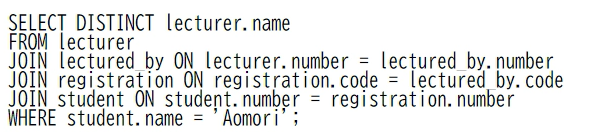
\includegraphics[width = 8cm]{sql1.png}
    \caption{課題1のSQL文}
\end{figure}
\subsection{解法}
課題1で最終的に出力する内容は教員名であるため,SELECT文にはlecturer.nameとした.\\
学生名が'Aomori'かどうかはstudentテーブル,履修しているかどうかはregistration,教授がどの科目を担当しているかはlectured\_byをそれぞれ参照する必要がある.
したがってlecturerと上記3つのテーブルを結合することにより学生名を参照すれば担当している教授名を参照できるようになる.
また,DISTINCTを入れた理由としては,'Aomori'という学生が同じ教授の授業を複数履修しており問い合わせの結果に同じ教授名が二回以上出力されないようにするためである.
\subsection{問い合わせの結果}
課題1の問い合わせの結果は以下の図2のようになる.
\begin{figure}[h]
    \centering
    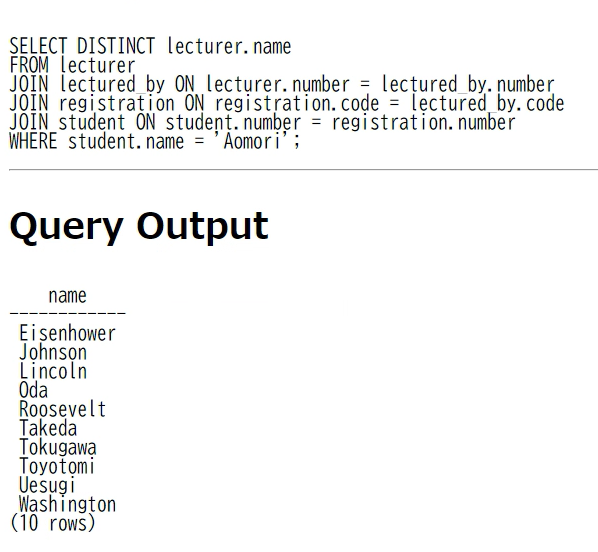
\includegraphics[width = 8cm]{1.png}
    \caption{問い合わせの結果}
\end{figure}
\section{課題2}
\subsection{課題内容}
履修者が最も少ない科目の科目番号と履修者数を求めよ.
\subsection{SQL文}
課題2のSQL文は以下の図3のようになる.
\begin{figure}[h]
    \centering
    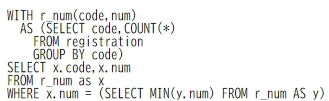
\includegraphics[width = 8cm]{sql2.png}
    \caption{課題2のSQL文}
\end{figure}
\subsection{解法}
課題2は,各科目の履修者数をそれぞれ求めてから比較する必要がある.したがって,まずGROUP BYとWITHを用いて一時的に各科目番号とその行数に関する表r\_numを作成する.行数はCOUNT(*)を用いて数えているが,
この理由は行数を履修者数としてみなしているためである.\\
そして作成したr\_numをxと名付けて参照し,xの履修者数の内最小値を副問い合わせから選択している.
副問い合わせでは再びr\_numを参照しており,ここではyと名付けている.
\subsection{問い合わせの結果}
課題1の問い合わせの結果は以下の図4のようになる.
\begin{figure}[h]
    \centering
    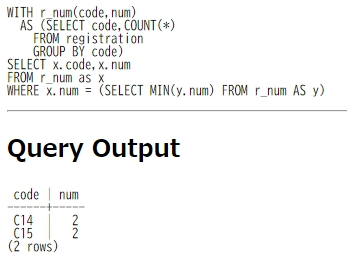
\includegraphics[width = 7cm]{2.png}
    \caption{問い合わせの結果}
\end{figure}
\section{課題3}
\subsection{課題内容}
科目ごとに成績の最も高い学生の成績と学生名を科目番号とともに求めよ.
\subsection{SQL文}
課題3のSQL文は以下の図5のようになる.
\begin{figure}[h]
    \centering
    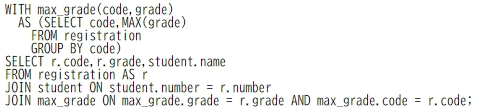
\includegraphics[width = 8cm]{sql3.png}
    \caption{課題3のSQL文}
\end{figure}
\subsection{解法}
課題3は,各科目の最高点を求めてから学生名と科目番号とともに出力する必要がある.したがって,課題2と同様にGROUP BYとWITHを用いて,一時的に
各科目番号とその科目の成績の最大値に関する表max\_gradeを作成する.科目番号と成績はregistrationを参照した.\\
課題3で出力するのは科目番号と成績の最大値,そして対応する学生名であるため,表を結合する.学生名が格納されているstudentとmax\_gradeは直接結合することができないため,registrationを用いて間接的に結合する.
したがって,JOINを使って図5のように結合している.
\subsection{問い合わせの結果}
課題3の問い合わせの結果は以下の図6のようになる.
\begin{figure}[h]
    \centering
    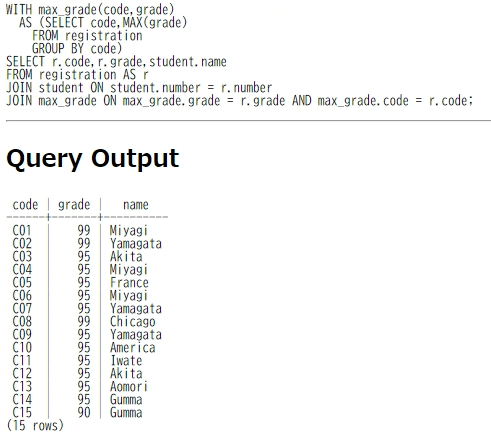
\includegraphics[width = 8cm]{3.png}
    \caption{問い合わせの結果}
\end{figure}
\section{課題4}
\subsection{課題内容}
必修の科目をすべて履修している学生の学籍番号を求めよ.
\subsection{SQL文}
課題4のSQL文は以下の図5のようになる.
\begin{figure}[h]
    \centering
    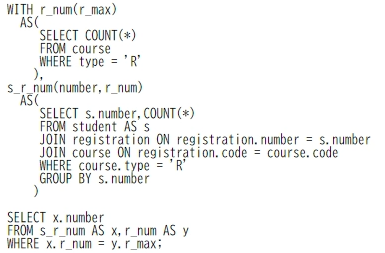
\includegraphics[width = 8cm]{sql4.png}
    \caption{課題4のSQL文}
\end{figure}
\subsection{解法}
課題4は,「各生徒が履修している必修科目の数」と「全ての必修科目の数」が一致している生徒が条件を満足すると考えた.
したがって,WITHを用いて二つの表を作成した.\\
\begin{itemize}
    \item 一つ目の表はr\_numであり,これは全ての必修科目の数を列として持つ.courseを参照しtypeが'R'である行数を数えることでこれを実現した.
    \item 二つ目の表はs\_r\_numであり,この表は学籍番号とその生徒が履修している必修科目の数を列として持つ.したがって,GROUP BYを用いて学籍番号ごとにグループ表を作成した.また,
    ここでは学籍番号を参照するためにstudentを参照しているが,必修科目の数を参照するためにtypeを用いる必要がある.つまりtypeとstudentを結合する必要があるが,これらには同じ列が存在しないため
    これら二つと同じ列を持つregistrationを用いて間接的に結合する.必修の科目はtypeが'R'であるのでWHERE文で指定した.
\end{itemize}
以上二つの表をFROM文に使用し,「各生徒が履修している必修科目の数」と「全ての必修科目の数」が一致している学籍番号を出力した.
\subsection{問い合わせの結果}
課題4の問い合わせの結果は以下の図6のようになる.
\begin{figure}[h]
    \centering
    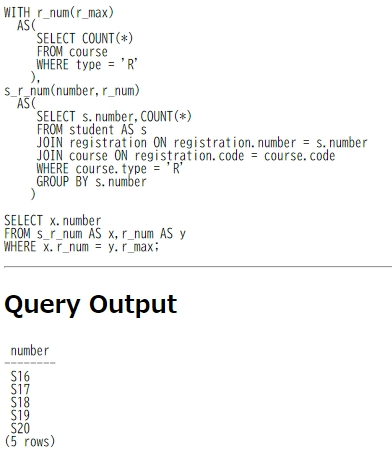
\includegraphics[width = 8cm]{4.png}
    \caption{問い合わせの結果}
\end{figure}
\section{感想}
今回の演習課題を通してWITHとGROUP BYの汎用性の高さを再認識することができた.最初はこれらの使い方をあまり理解できず,
かなり苦戦していたので今回の課題を終わらせるのにかなり時間がかかってしまった.前回と今回の課題を通して,SQLの書き方や考え方等にはかなり慣れることができたので将来的に使用する際にはこの経験を活かしていきたいと思う.
\end{document}